% !TEX TS-program = pdflatex
\documentclass[11pt]{article}

% -------------------- Packages --------------------
\usepackage[a4paper,margin=1in]{geometry}
\usepackage{amsmath,amssymb}
\usepackage[T1]{fontenc}
\usepackage{lmodern}
\usepackage{xcolor}
\usepackage{tcolorbox}
\tcbuselibrary{skins,breakable}
\usepackage{enumitem}
\usepackage{hyperref}
\usepackage{tikz}
\usetikzlibrary{calc,arrows.meta}

\pagestyle{empty}

% -------------------- Dark Theme Colors --------------------
\definecolor{bg}{HTML}{000000}
\definecolor{pairbg}{HTML}{121212}
\definecolor{solbg}{HTML}{0A0A0A}
\definecolor{border}{HTML}{2A2A2A}
\definecolor{text}{HTML}{FFFFFF}
\definecolor{muted}{HTML}{C9CDD3}
\definecolor{gold}{HTML}{FFD700}
\definecolor{green}{HTML}{4ADE80}
\definecolor{cyan}{HTML}{38BDF8}

\pagecolor{bg}
\color{text}

\hypersetup{
  colorlinks=true,
  linkcolor=cyan,
  urlcolor=cyan
}

\setlength{\parindent}{0pt}
\setlength{\parskip}{10pt}

% Help LaTeX avoid overfull lines globally
\sloppy
\setlength{\emergencystretch}{3em}

\setlist[itemize]{left=1.4em,itemsep=6pt,topsep=6pt}
\setlist[enumerate]{left=1.6em,itemsep=4pt,topsep=4pt}

% -------------------- tcolorbox Base --------------------
\tcbset{
  enhanced,
  breakable,
  arc=12pt,
  boxrule=0.8pt,
  left=14pt,right=14pt,top=12pt,bottom=12pt
}

\newtcolorbox{QAPair}[1]{%
  colback=pairbg,
  colbacklower=solbg,
  colframe=border,
  coltext=text,
  title=\textcolor{gold}{\bfseries #1},
  fonttitle=\bfseries,
  coltitle=text,
  segmentation style={draw=border, dashed, line width=0.6pt},
  before upper=\raggedright,
  before lower=\raggedright
}

\newtcolorbox{QuickBox}{%
  colback=pairbg,
  colframe=cyan,
  coltext=text,
  fontupper=\color{text}\raggedright,
  borderline north={4pt}{0pt}{cyan},
  arc=14pt,
  boxrule=0.8pt
}

% Helper for step headings
\newcommand{\Step}[1]{\textcolor{muted}{\textbf{Step #1:}}}

% Small centered diagram block (for step-by-step visuals)
\newenvironment{StepDiagram}{\par\medskip\begin{center}}{\end{center}\medskip}

% TikZ styles
\tikzset{
  base/.style={draw=text, line width=0.9pt, line cap=round, line join=round},
  new/.style={draw=cyan, line width=1.2pt, line cap=round, line join=round},
  help/.style={draw=muted, dashed, line width=0.9pt},
  medline/.style={draw=gold, line width=1.2pt},
  dot/.style={circle, fill=text, inner sep=1.2pt},
  lab/.style={text=text, font=\small},
  labs/.style={text=text, font=\scriptsize},
  labm/.style={text=muted, font=\small},
}

% A tiny "equation diagram" (boxed) so every algebra step has a visual too
\newcommand{\EqDiagram}[1]{%
\begin{StepDiagram}
\begin{tikzpicture}
\node[draw=border, rounded corners=10pt, inner sep=8pt, text=text, align=left, text width=0.87\linewidth] {#1};
\end{tikzpicture}
\end{StepDiagram}
}

% ------------------------------------------------------------
% Macro: Horizontal Box & Whisker (numeric) with clean mapping
% Args: min, q1, med, q3, max, axisMin, axisMax, label
% ------------------------------------------------------------
\newcommand{\HBoxWhisker}[8]{%
\begin{tikzpicture}
  \def\minv{#1}\def\qone{#2}\def\med{#3}\def\qthr{#4}\def\maxv{#5}
  \def\Amin{#6}\def\Amax{#7}
  \def\W{10} % plot width in "tikz units"

  \pgfmathsetmacro{\xmin}{(\minv-\Amin)/(\Amax-\Amin)*\W}
  \pgfmathsetmacro{\xqone}{(\qone-\Amin)/(\Amax-\Amin)*\W}
  \pgfmathsetmacro{\xmed}{(\med-\Amin)/(\Amax-\Amin)*\W}
  \pgfmathsetmacro{\xqthr}{(\qthr-\Amin)/(\Amax-\Amin)*\W}
  \pgfmathsetmacro{\xmax}{(\maxv-\Amin)/(\Amax-\Amin)*\W}

  % axis
  \draw[base] (0,0) -- (\W,0);
  \node[labs, fill=pairbg, inner sep=1pt] at (0,-0.55) {$\Amin$};
  \node[labs, fill=pairbg, inner sep=1pt] at (\W,-0.55) {$\Amax$};

  % whiskers
  \draw[new] (\xmin,0) -- (\xqone,0);
  \draw[new] (\xqthr,0) -- (\xmax,0);
  \draw[new] (\xmin,0.28) -- (\xmin,-0.28);
  \draw[new] (\xmax,0.28) -- (\xmax,-0.28);

  % box
  \draw[new, fill=pairbg] (\xqone,0.45) rectangle (\xqthr,-0.45);

  % median
  \draw[medline] (\xmed,0.45) -- (\xmed,-0.45);

  % labels (placed above; filled to avoid line-through)
  \node[labs, fill=pairbg, inner sep=1pt] at (\xmin,0.78) {min};
  \node[labs, fill=pairbg, inner sep=1pt] at (\xqone,0.78) {$Q_1$};
  \node[labs, fill=pairbg, inner sep=1pt] at (\xmed,0.78) {med};
  \node[labs, fill=pairbg, inner sep=1pt] at (\xqthr,0.78) {$Q_3$};
  \node[labs, fill=pairbg, inner sep=1pt] at (\xmax,0.78) {max};

  % title
  \node[lab] at (\W/2,1.35) {#8};
\end{tikzpicture}
}

% ------------------------------------------------------------
% Macro: Tiny trend scatter (for correlation quick formula)
% ------------------------------------------------------------
\newcommand{\TinyTrend}[1]{%
\begin{tikzpicture}[scale=0.9]
  \draw[base,->] (0,0) -- (2.8,0) node[labs,below] {x};
  \draw[base,->] (0,0) -- (0,2.2) node[labs,left] {y};
  \ifx#1p
    \foreach \x/\y in {0.5/0.6,0.8/0.9,1.2/1.2,1.6/1.5,2.1/1.8} {\node[dot] at (\x,\y) {};}
    \draw[new] (0.3,0.4) -- (2.4,1.95);
    \node[labs, fill=pairbg, inner sep=1pt] at (1.55,2.05) {positive};
  \fi
  \ifx#1n
    \foreach \x/\y in {0.5/1.8,0.8/1.55,1.2/1.25,1.6/0.95,2.1/0.7} {\node[dot] at (\x,\y) {};}
    \draw[new] (0.3,1.95) -- (2.4,0.55);
    \node[labs, fill=pairbg, inner sep=1pt] at (1.55,2.05) {negative};
  \fi
  \ifx#1z
    \foreach \x/\y in {0.6/1.2,0.9/0.8,1.2/1.5,1.6/0.9,2.1/1.3} {\node[dot] at (\x,\y) {};}
    \node[labs, fill=pairbg, inner sep=1pt] at (1.55,2.05) {no clear};
  \fi
\end{tikzpicture}
}

% ============================================================
\begin{document}

\begin{center}
{\LARGE\bfseries \textcolor{gold}{Exercise 12.2 --- Solutions}}\\[-2pt]
\end{center}

% -------------------- Quick formulas + diagram PER LINE --------------------
\begin{QuickBox}
{\color{cyan}\bfseries Quick formulas (Box plots, IQR \& Correlation)}\par\medskip

\begin{itemize}
\item \textbf{Interquartile range (IQR):}\quad $\mathrm{IQR}=Q_3-Q_1$.
\begin{StepDiagram}
\HBoxWhisker{10}{30}{50}{70}{90}{0}{100}{IQR is the width of the box ($Q_1\to Q_3$)}
\end{StepDiagram}

\item \textbf{Percent above $Q_3$:}\quad $25\%$ of data lies above $Q_3$ (top quartile).
\begin{StepDiagram}

\begin{tikzpicture}
  \draw[base] (0,0) rectangle (8,1.2);
  \draw[help] (2,0) -- (2,1.2);
  \draw[help] (4,0) -- (4,1.2);
  \draw[help] (6,0) -- (6,1.2);
  \fill[cyan, opacity=0.25] (6,0) rectangle (8,1.2);
  \node[labs] at (1,0.6) {$25\%$};
  \node[labs] at (3,0.6) {$25\%$};
  \node[labs] at (5,0.6) {$25\%$};
  \node[labs, fill=pairbg, inner sep=1pt] at (7,0.6) {$25\%$ above $Q_3$};
  \node[labs] at (2,-0.35) {$Q_1$};
  \node[labs] at (4,-0.35) {median};
  \node[labs] at (6,-0.35) {$Q_3$};
\end{tikzpicture}
\end{StepDiagram}

\item \textbf{Correlation from a scatter plot:} upward trend $\Rightarrow$ positive; downward trend $\Rightarrow$ negative.
\begin{StepDiagram}
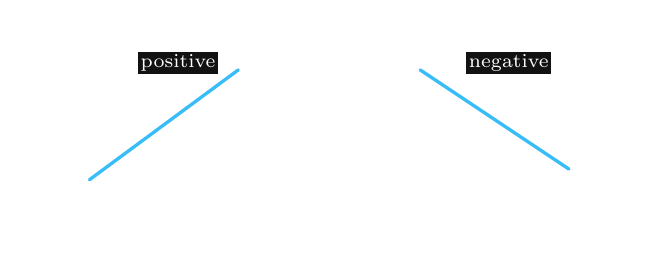
\begin{tikzpicture}
\node at (0,0) {\TinyTrend{p}};
\node at (4.2,0) {\TinyTrend{n}};
\end{tikzpicture}
\end{StepDiagram}

\item \textbf{Line of best fit:} a straight line that passes through the middle of points (rough balance above \& below).
\begin{StepDiagram}
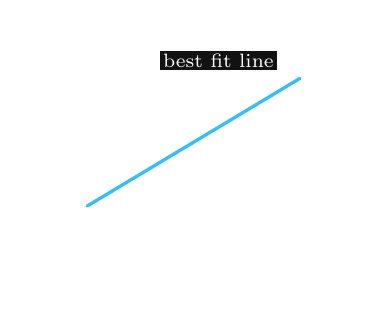
\begin{tikzpicture}[scale=0.9]
  \draw[base,->] (0,0) -- (4.0,0) node[labs,below] {x};
  \draw[base,->] (0,0) -- (0,3.0) node[labs,left] {y};
  \foreach \x/\y in {0.6/0.8,1.1/1.0,1.5/1.4,2.1/1.7,2.6/2.1,3.2/2.4} {\node[dot] at (\x,\y) {};}
  \draw[new] (0.4,0.7) -- (3.4,2.5);
  \node[labs, fill=pairbg, inner sep=1pt] at (2.25,2.75) {best fit line};
\end{tikzpicture}
\end{StepDiagram}
\end{itemize}
\end{QuickBox}

% ============================================================
% Q1
\begin{QAPair}{Question 1}
\textcolor{gold}{\bfseries Question:} A mechanical engineer wants to analyze the relationship between the mass of a car and its fuel efficiency.
Show the data by box and whisker plots.

\smallskip
\textbf{Mass (kg):} min $1100$, $Q_1=1200$, median $1500$, $Q_3=1700$, max $2000$.

\textbf{Fuel efficiency (km/l):} max $24$, $Q_1=20$, median $14$, $Q_3=12$, min $10$.

\smallskip
(a) Find IQR \quad (b) Type of correlation \quad (c) Conclusion.
\tcblower
\textcolor{green}{\bfseries Answer:}\par

\Step{1} Write the five-number summaries (in increasing order).
\[
\text{Mass: }(1100,\,1200,\,1500,\,1700,\,2000),\qquad
\text{Fuel: }(10,\,12,\,14,\,20,\,24).
\]
\EqDiagram{Put fuel efficiency in order: $10<12<14<20<24$ (so $Q_1=12,\ Q_3=20$ for fuel).}

\Step{2} Draw the box and whisker plot for \textbf{Mass (kg)}.
\begin{StepDiagram}
\HBoxWhisker{1100}{1200}{1500}{1700}{2000}{1000}{2100}{Mass (kg)}
\end{StepDiagram}

\Step{3} Mass IQR:
\[
\mathrm{IQR}_{\text{mass}}=Q_3-Q_1=1700-1200=500\text{ kg}.
\]
\EqDiagram{$\mathrm{IQR}_{\text{mass}}=1700-1200=500\text{ kg}$}

\Step{4} Draw the box and whisker plot for \textbf{Fuel efficiency (km/l)}.
\begin{StepDiagram}
\HBoxWhisker{10}{12}{14}{20}{24}{8}{26}{Fuel efficiency (km/l)}
\end{StepDiagram}

\Step{5} Fuel-efficiency IQR:
\[
\mathrm{IQR}_{\text{fuel}}=Q_3-Q_1=20-12=8\text{ km/l}.
\]
\EqDiagram{$\mathrm{IQR}_{\text{fuel}}=20-12=8\text{ km/l}$}

\Step{6} Correlation \& conclusion: when mass increases, fuel efficiency decreases $\Rightarrow$ \textbf{negative correlation}.
\begin{StepDiagram}

\begin{tikzpicture}
  \draw[base,->] (0,0) -- (9,0);
  \node[lab] at (1.0,0.55) {Mass $\uparrow$};
  \node[lab] at (7.8,0.55) {Fuel efficiency $\downarrow$};
  \draw[new,->] (2.2,0.25) -- (6.8,0.25);
  \node[labs, fill=pairbg, inner sep=1pt] at (4.5,-0.55) {negative relationship};
\end{tikzpicture}
\end{StepDiagram}

\[
\boxed{\mathrm{IQR}_{\text{mass}}=500\text{ kg},\ \mathrm{IQR}_{\text{fuel}}=8\text{ km/l},\ \text{Correlation: Negative.}}
\]
\[
\boxed{\text{Conclusion: Heavier cars generally have lower fuel efficiency.}}
\]
\end{QAPair}

% ============================================================
% Q2
\begin{QAPair}{Question 2}
\textcolor{gold}{\bfseries Question:} The adjoining box \& whisker plot shows wages for part-time and full-time employees.

(a) Median wages for full-time employees? \quad
(b) Minimum and maximum wages for part-time employees?

(c) IQR for full-time dataset? \quad
(d) IQR for part-time dataset? \quad
(e) What type of correlation is observed in both datasets?
\tcblower
\textcolor{green}{\bfseries Answer:}\par

\Step{1} Re-draw the two boxplots on a clear axis (values read from the given diagram).
\begin{StepDiagram}
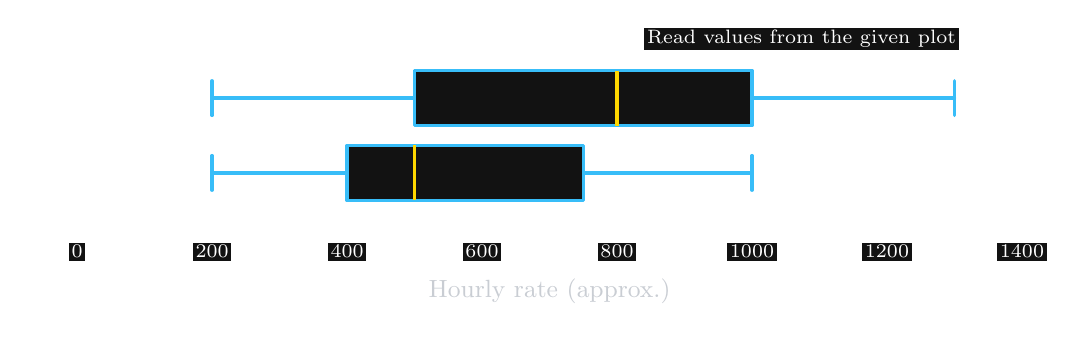
\begin{tikzpicture}
  % axis
  \def\W{12}
  \def\Amin{0}
  \def\Amax{1400}
  \draw[base] (0,0) -- (\W,0);
  \foreach \t in {0,200,400,600,800,1000,1200,1400}{
    \pgfmathsetmacro{\x}{(\t-\Amin)/(\Amax-\Amin)*\W}
    \draw[base] (\x,0.12)--(\x,-0.12);
    \node[labs, fill=pairbg, inner sep=1pt] at (\x,-0.45) {\t};
  }
  \node[labm] at (\W/2,-0.95) {Hourly rate (approx.)};

  % y positions
  \def\yF{1.5}
  \def\yP{0.55}

  % FULL-TIME (F): min 200, Q1 500, med 800, Q3 1000, max 1300
  \foreach \v/\name in {200/min,500/Q1,800/med,1000/Q3,1300/max}{
    \pgfmathsetmacro{\xv}{(\v-\Amin)/(\Amax-\Amin)*\W}
  }
  \pgfmathsetmacro{\xFmin}{(200-\Amin)/(\Amax-\Amin)*\W}
  \pgfmathsetmacro{\xFqone}{(500-\Amin)/(\Amax-\Amin)*\W}
  \pgfmathsetmacro{\xFmed}{(800-\Amin)/(\Amax-\Amin)*\W}
  \pgfmathsetmacro{\xFqthr}{(1000-\Amin)/(\Amax-\Amin)*\W}
  \pgfmathsetmacro{\xFmax}{(1300-\Amin)/(\Amax-\Amin)*\W}

  \node[lab] at (-0.4,\yF) {F};
  \draw[new] (\xFmin,\yF) -- (\xFqone,\yF);
  \draw[new] (\xFqthr,\yF) -- (\xFmax,\yF);
  \draw[new] (\xFmin,\yF+0.22) -- (\xFmin,\yF-0.22);
  \draw[new] (\xFmax,\yF+0.22) -- (\xFmax,\yF-0.22);
  \draw[new, fill=pairbg] (\xFqone,\yF+0.35) rectangle (\xFqthr,\yF-0.35);
  \draw[medline] (\xFmed,\yF+0.35) -- (\xFmed,\yF-0.35);

  % PART-TIME (P): min 200, Q1 400, med 500, Q3 750, max 1000
  \pgfmathsetmacro{\xPmin}{(200-\Amin)/(\Amax-\Amin)*\W}
  \pgfmathsetmacro{\xPqone}{(400-\Amin)/(\Amax-\Amin)*\W}
  \pgfmathsetmacro{\xPmed}{(500-\Amin)/(\Amax-\Amin)*\W}
  \pgfmathsetmacro{\xPqthr}{(750-\Amin)/(\Amax-\Amin)*\W}
  \pgfmathsetmacro{\xPmax}{(1000-\Amin)/(\Amax-\Amin)*\W}

  \node[lab] at (-0.4,\yP) {P};
  \draw[new] (\xPmin,\yP) -- (\xPqone,\yP);
  \draw[new] (\xPqthr,\yP) -- (\xPmax,\yP);
  \draw[new] (\xPmin,\yP+0.22) -- (\xPmin,\yP-0.22);
  \draw[new] (\xPmax,\yP+0.22) -- (\xPmax,\yP-0.22);
  \draw[new, fill=pairbg] (\xPqone,\yP+0.35) rectangle (\xPqthr,\yP-0.35);
  \draw[medline] (\xPmed,\yP+0.35) -- (\xPmed,\yP-0.35);

  \node[labs, fill=pairbg, inner sep=1pt] at (9.2,2.25) {Read values from the given plot};
\end{tikzpicture}
\end{StepDiagram}

\Step{2} (a) The \textbf{median} wage for full-time employees is the vertical line inside the box:
\[
\boxed{\text{Median (Full-time)}\approx 800.}
\]
\begin{StepDiagram}

\begin{tikzpicture}
  \node[labm, align=center] at (0,0) {Median is the middle line inside the box};
  \draw[new, fill=pairbg] (1.0,-0.3) rectangle (5.0,0.3);
  \draw[medline] (3.4,-0.3) -- (3.4,0.3);
  \node[labs, fill=pairbg, inner sep=1pt] at (3.4,0.65) {median};
\end{tikzpicture}
\end{StepDiagram}

\Step{3} (b) Part-time minimum and maximum are at the ends of whiskers:
\[
\boxed{\text{Min (Part-time)}\approx 200,\qquad \text{Max (Part-time)}\approx 1000.}
\]
\begin{StepDiagram}
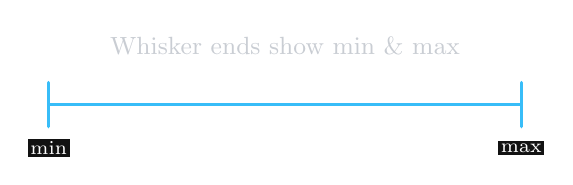
\begin{tikzpicture}
  \draw[new] (0,0) -- (6,0);
  \draw[new] (0,0.28)--(0,-0.28);
  \draw[new] (6,0.28)--(6,-0.28);
  \node[labs, fill=pairbg, inner sep=1pt] at (0,-0.55) {min};
  \node[labs, fill=pairbg, inner sep=1pt] at (6,-0.55) {max};
  \node[labm] at (3,0.75) {Whisker ends show min \& max};
\end{tikzpicture}
\end{StepDiagram}

\Step{4} (c) Full-time IQR:
\[
\mathrm{IQR}_F=Q_3-Q_1\approx 1000-500=500.
\]
\EqDiagram{$\mathrm{IQR}_F\approx 1000-500=500$}

\Step{5} (d) Part-time IQR:
\[
\mathrm{IQR}_P=Q_3-Q_1\approx 750-400=350.
\]
\EqDiagram{$\mathrm{IQR}_P\approx 750-400=350$}

\Step{6} (e) Both datasets show wages generally shifting to higher values for full-time than part-time (part-time box is left of full-time box).
This indicates a \textbf{positive association} (higher job type $\Rightarrow$ higher wage).
\begin{StepDiagram}
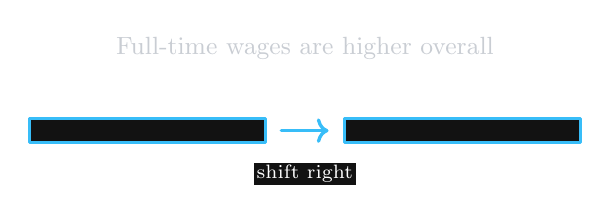
\begin{tikzpicture}
  \draw[new, fill=pairbg] (0.6,0.15) rectangle (3.6,-0.15);
  \draw[new, fill=pairbg] (4.6,0.15) rectangle (7.6,-0.15);
  \node[labs] at (2.1,0.55) {P};
  \node[labs] at (6.1,0.55) {F};
  \draw[new,->] (3.8,0) -- (4.4,0);
  \node[labs, fill=pairbg, inner sep=1pt] at (4.1,-0.55) {shift right};
  \node[labm] at (4.1,1.05) {Full-time wages are higher overall};
\end{tikzpicture}
\end{StepDiagram}

\[
\boxed{\text{(a) }800\ \ \text{(b) }200,\,1000\ \ \text{(c) }500\ \ \text{(d) }350\ \ \text{(e) Positive association.}}
\]
\end{QAPair}

% ============================================================
% Q3
\begin{QAPair}{Question 3}
\textcolor{gold}{\bfseries Question:} Maryam wants to investigate the relationship between rainfall and number of flowers blooming.
Draw the scatter diagram using:

\[
\text{Rain (inch): }2,\ 4,\ 6,\ 8,\ 10
\qquad
\text{No. of flowers: }10,\ 22,\ 55,\ 70,\ 80
\]
(a) Draw a line of best fit. \quad (b) Comment on type of correlation.
\tcblower
\textcolor{green}{\bfseries Answer:}\par

\Step{1} Plot the points on a scatter diagram.
\begin{StepDiagram}
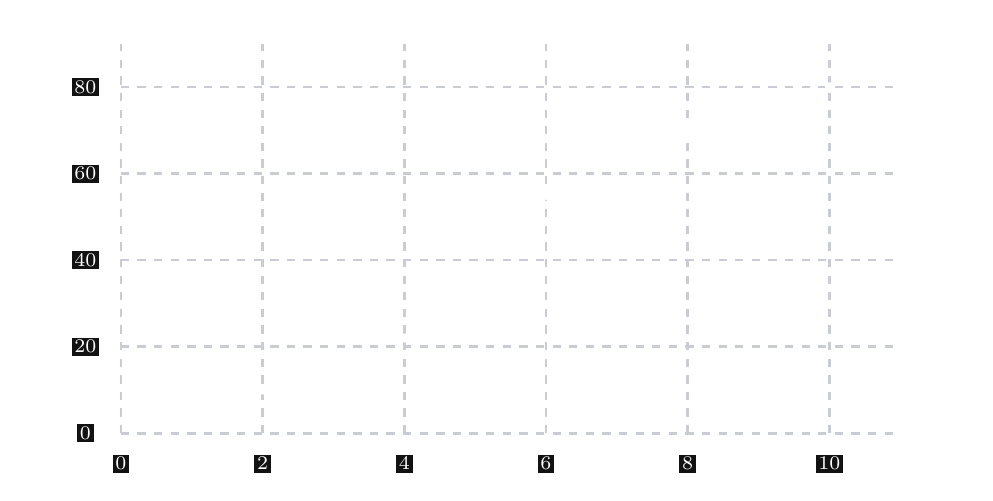
\begin{tikzpicture}[x=0.9cm,y=0.055cm]
  \draw[base,->] (0,0) -- (11,0) node[labs,below] {Rain (inch)};
  \draw[base,->] (0,0) -- (0,90) node[labs,left] {Flowers};
  \foreach \x in {0,2,4,6,8,10}{
    \draw[help] (\x,0) -- (\x,90);
    \node[labs, fill=pairbg, inner sep=1pt] at (\x,-7) {\x};
  }
  \foreach \y in {0,20,40,60,80}{
    \draw[help] (0,\y) -- (11,\y);
    \node[labs, fill=pairbg, inner sep=1pt] at (-0.5,\y) {\y};
  }
  \foreach \x/\y in {2/10,4/22,6/55,8/70,10/80}{
    \node[dot] at (\x,\y) {};
  }
\end{tikzpicture}
\end{StepDiagram}

\Step{2} Draw a line of best fit (passing through the middle of the points).
\begin{StepDiagram}
\begin{tikzpicture}[x=0.9cm,y=0.055cm]
  \draw[base,->] (0,0) -- (11,0) node[labs,below] {Rain};
  \draw[base,->] (0,0) -- (0,90) node[labs,left] {Flowers};
  \foreach \x/\y in {2/10,4/22,6/55,8/70,10/80}{\node[dot] at (\x,\y) {};}
  \draw[new] (1.5,5) -- (10.5,85);
  \node[labs, fill=pairbg, inner sep=1pt] at (7.7,84) {best fit};
\end{tikzpicture}
\end{StepDiagram}

\Step{3} Since the points rise as rainfall increases, the correlation is \textbf{positive}.
\begin{StepDiagram}
\TinyTrend{p}
\end{StepDiagram}

\[
\boxed{\text{Correlation: Positive.}}
\]
\end{QAPair}

% ============================================================
% Q4
\begin{QAPair}{Question 4}
\textcolor{gold}{\bfseries Question:} Given scatter diagram shows relation between practice time and marks obtained in math test.
(a) Find type of correlation.\quad (b) Draw a line of best fit.
\tcblower
\textcolor{green}{\bfseries Answer:}\par

\Step{1} Re-draw a clean scatter plot (approximate points as shown).
\begin{StepDiagram}
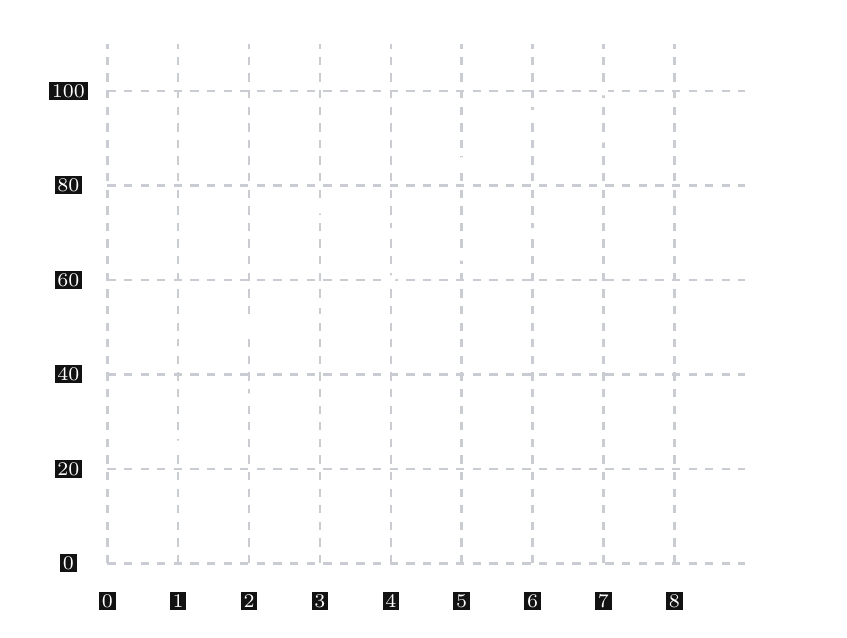
\begin{tikzpicture}[x=0.9cm,y=0.06cm]
  \draw[base,->] (0,0) -- (9,0) node[labs,below] {Practice time};
  \draw[base,->] (0,0) -- (0,110) node[labs,left] {Marks};
  \foreach \x in {0,1,2,3,4,5,6,7,8}{
    \draw[help] (\x,0) -- (\x,110);
    \node[labs, fill=pairbg, inner sep=1pt] at (\x,-8) {\x};
  }
  \foreach \y in {0,20,40,60,80,100}{
    \draw[help] (0,\y) -- (9,\y);
    \node[labs, fill=pairbg, inner sep=1pt] at (-0.55,\y) {\y};
  }

  % approx points (from the diagram)
  \foreach \x/\y in {
    1/25,1/45,2/35,2/50,3/55,3/75,4/60,4/70,5/65,5/85,6/70,6/95,7/90,7/100
  }{
    \node[dot] at (\x,\y) {};
  }
\end{tikzpicture}
\end{StepDiagram}

\Step{2} Draw a line of best fit (upward sloping).
\begin{StepDiagram}
\begin{tikzpicture}[x=0.9cm,y=0.06cm]
  \draw[base,->] (0,0) -- (9,0) node[labs,below] {Time};
  \draw[base,->] (0,0) -- (0,110) node[labs,left] {Marks};

  \foreach \x/\y in {
    1/25,1/45,2/35,2/50,3/55,3/75,4/60,4/70,5/65,5/85,6/70,6/95,7/90,7/100
  }{\node[dot] at (\x,\y) {};}

  \draw[new] (0.8,25) -- (7.6,100);
  \node[labs, fill=pairbg, inner sep=1pt] at (6.0,103) {best fit};
\end{tikzpicture}
\end{StepDiagram}

\Step{3} The points generally rise as time increases, so the correlation is \textbf{positive}.
\begin{StepDiagram}
\TinyTrend{p}
\end{StepDiagram}

\[
\boxed{\text{Correlation: Positive.}}
\]
\end{QAPair}

% ============================================================
% Q5
\begin{QAPair}{Question 5}
\textcolor{gold}{\bfseries Question:} Draw the scatter diagram for the data showing relationship between AQI and sick days:

\[
\text{AQI: }20,40,60,80,100,120,10,30,50,70
\]
\[
\text{Sick days: }5,18,25,40,60,80,3,15,20,27
\]
Find correlation and what does this suggest?
\tcblower
\textcolor{green}{\bfseries Answer:}\par

\Step{1} Plot the points $(\text{AQI},\text{sick days})$.
\begin{StepDiagram}
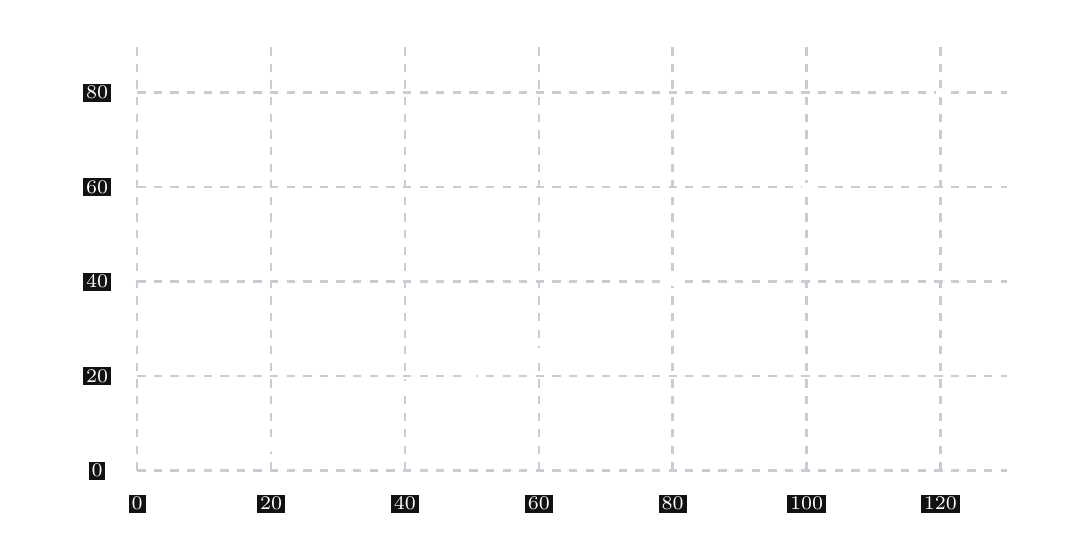
\begin{tikzpicture}[x=0.085cm,y=0.06cm]
  \draw[base,->] (0,0) -- (130,0) node[labs,below] {AQI};
  \draw[base,->] (0,0) -- (0,90) node[labs,left] {Sick days};

  \foreach \x in {0,20,40,60,80,100,120}{
    \draw[help] (\x,0) -- (\x,90);
    \node[labs, fill=pairbg, inner sep=1pt] at (\x,-7) {\x};
  }
  \foreach \y in {0,20,40,60,80}{
    \draw[help] (0,\y) -- (130,\y);
    \node[labs, fill=pairbg, inner sep=1pt] at (-6,\y) {\y};
  }

  \foreach \x/\y in {20/5,40/18,60/25,80/40,100/60,120/80,10/3,30/15,50/20,70/27}{
    \node[dot] at (\x,\y) {};
  }
\end{tikzpicture}
\end{StepDiagram}

\Step{2} Draw a best-fit line (clear upward trend).
\begin{StepDiagram}
\begin{tikzpicture}[x=0.085cm,y=0.06cm]
  \draw[base,->] (0,0) -- (130,0) node[labs,below] {AQI};
  \draw[base,->] (0,0) -- (0,90) node[labs,left] {Sick days};

  \foreach \x/\y in {20/5,40/18,60/25,80/40,100/60,120/80,10/3,30/15,50/20,70/27}{
    \node[dot] at (\x,\y) {};
  }

  \draw[new] (5,2) -- (125,83);
  \node[labs, fill=pairbg, inner sep=1pt] at (95,86) {best fit};
\end{tikzpicture}
\end{StepDiagram}

\Step{3} Correlation is \textbf{strong positive}. Suggestion: higher pollution level $\Rightarrow$ more sick days.
\begin{StepDiagram}
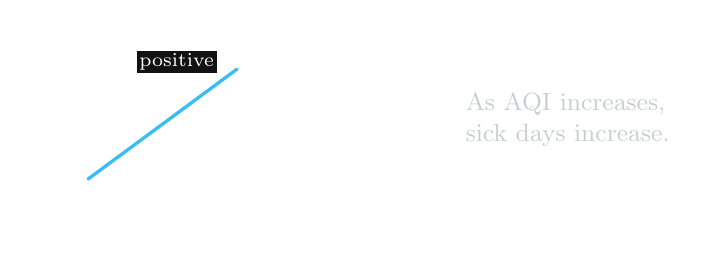
\begin{tikzpicture}
  \node[lab] at (0,0) {\TinyTrend{p}};
  \node[labm, align=left] at (5.2,0.2) {As AQI increases,\\ sick days increase.};
\end{tikzpicture}
\end{StepDiagram}

\[
\boxed{\text{Correlation: Strong positive. Suggests pollution increases sick days.}}
\]
\end{QAPair}

% ============================================================
% Q6
\begin{QAPair}{Question 6}
\textcolor{gold}{\bfseries Question:} A teacher wants to analyze the test scores of her students.
Draw a box and whisker plot to show a median score of $75$, a first quartile of $60$, and a third quartile of $85$.

Find:
(a) What percentage of students scored above $85$? \quad
(b) IQR
\tcblower
\textcolor{green}{\bfseries Answer:}\par

\Step{1} Draw the box plot using $Q_1=60$, median $=75$, $Q_3=85$.
(Whiskers represent min/max but are not given, so we show them as unlabeled ends.)
\begin{StepDiagram}
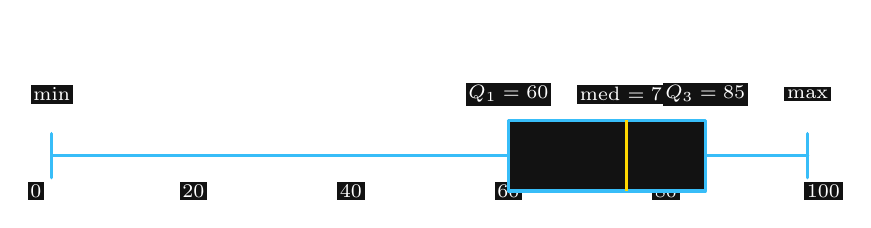
\begin{tikzpicture}
  \def\Amin{0}\def\Amax{100}\def\W{10}
  \def\qone{60}\def\med{75}\def\qthr{85}
  \pgfmathsetmacro{\xqone}{(\qone-\Amin)/(\Amax-\Amin)*\W}
  \pgfmathsetmacro{\xmed}{(\med-\Amin)/(\Amax-\Amin)*\W}
  \pgfmathsetmacro{\xqthr}{(\qthr-\Amin)/(\Amax-\Amin)*\W}

  % axis
  \draw[base] (0,0) -- (\W,0);
  \foreach \t in {0,20,40,60,80,100}{
    \pgfmathsetmacro{\x}{(\t-\Amin)/(\Amax-\Amin)*\W}
    \draw[base] (\x,0.12)--(\x,-0.12);
    \node[labs, fill=pairbg, inner sep=1pt] at (\x,-0.45) {\t};
  }

  % "unknown" whiskers (shown but not numbered)
  \draw[new] (0.2,0) -- (\xqone,0);
  \draw[new] (\xqthr,0) -- (9.8,0);
  \draw[new] (0.2,0.28) -- (0.2,-0.28);
  \draw[new] (9.8,0.28) -- (9.8,-0.28);
  \node[labs, fill=pairbg, inner sep=1pt] at (0.2,0.78) {min};
  \node[labs, fill=pairbg, inner sep=1pt] at (9.8,0.78) {max};

  % box and median
  \draw[new, fill=pairbg] (\xqone,0.45) rectangle (\xqthr,-0.45);
  \draw[medline] (\xmed,0.45) -- (\xmed,-0.45);

  % labels
  \node[labs, fill=pairbg, inner sep=1pt] at (\xqone,0.78) {$Q_1=60$};
  \node[labs, fill=pairbg, inner sep=1pt] at (\xmed,0.78) {med $=75$};
  \node[labs, fill=pairbg, inner sep=1pt] at (\xqthr,0.78) {$Q_3=85$};

  \node[lab] at (\W/2,1.35) {Scores box plot (key quartiles given)};
\end{tikzpicture}
\end{StepDiagram}

\Step{2} (a) Since $Q_3=85$, the top quartile lies above $85$:
\[
\boxed{25\% \text{ of students scored above }85.}
\]
\begin{StepDiagram}

\begin{tikzpicture}
  \fill[cyan, opacity=0.20] (6,0) rectangle (8,1.1);
  \draw[base] (0,0) rectangle (8,1.1);
  \draw[help] (2,0)--(2,1.1);
  \draw[help] (4,0)--(4,1.1);
  \draw[help] (6,0)--(6,1.1);
  \node[labs] at (1,0.55) {$25\%$};
  \node[labs] at (3,0.55) {$25\%$};
  \node[labs] at (5,0.55) {$25\%$};
  \node[labs, fill=pairbg, inner sep=1pt] at (7,0.55) {$25\%$ above $Q_3$};
\end{tikzpicture}
\end{StepDiagram}

\Step{3} (b) IQR:
\[
\mathrm{IQR}=Q_3-Q_1=85-60=25.
\]
\EqDiagram{$\mathrm{IQR}=85-60=25$}

\[
\boxed{(a)\ 25\%\qquad (b)\ \mathrm{IQR}=25.}
\]
\end{QAPair}

\end{document}
